\section{Capítulo 1 -- Lógica, algoritmos e o computador}

Programar é, antes de tudo, organizar o pensamento. Antes de escrever uma única linha em uma linguagem de programação, é preciso entender o problema, decidir quais passos o resolvem e em que ordem executá-los. Neste capítulo você vai conhecer as ideias que sustentam todo o resto da disciplina: o que é lógica, o que é um algoritmo, como um computador executa instruções e duas formas de escrever algoritmos antes de programar, o \textbf{fluxograma} e o \textbf{Portugol}. No final, vai ver o mesmo algoritmo escrito em C++, a linguagem que usaremos ao longo da apostila.

\subsection{1.1 Lógica}

\textbf{Lógica} é o estudo das formas corretas de raciocinar: como chegar a conclusões verdadeiras a partir de informações verdadeiras. Você a usa o tempo todo sem perceber. Se o aplicativo diz que vai chover e você vai sair, então leva o guarda-chuva. Se o saldo da conta é menor que o preço, então a compra não passa.

O ponto de partida da lógica é a \textbf{proposição}: uma frase que pode ser classificada como verdadeira ou falsa, mas não as duas coisas ao mesmo tempo. ``A nota é maior ou igual a 6'' é uma proposição; ``Estude para a prova!'' não é, porque não faz sentido perguntar se é verdadeira.

Proposições podem ser combinadas com três conectivos, que vão aparecer em todos os programas que você escrever:

\begin{itemize}
  \item \textbf{E}: ``tem nota maior ou igual a 6 \textbf{e} frequência maior ou igual a 75\%'' só é verdadeira quando as duas partes são verdadeiras.
  \item \textbf{OU}: ``paga meia entrada se é estudante \textbf{ou} tem mais de 60 anos'' é verdadeira quando pelo menos uma das partes é verdadeira.
  \item \textbf{NÃO}: inverte o valor. Se ``a porta está aberta'' é verdadeira, ``a porta \textbf{não} está aberta'' é falsa.
\end{itemize}

A \textbf{tabela-verdade} mostra o resultado para todas as combinações possíveis. Nela, V significa verdadeiro e F, falso:

\begin{center}
\begin{tabular}{@{}p{0.12\linewidth}p{0.12\linewidth}p{0.16\linewidth}p{0.18\linewidth}p{0.16\linewidth}@{}}
\toprule
\rowcolor{headergray}
\tblheader{A} & \tblheader{B} & \tblheader{A E B} & \tblheader{A OU B} & \tblheader{NÃO A} \\
\midrule
V & V & V & V & F \\
\rowcolor{rowgray} V & F & F & V & F \\
F & V & F & V & V \\
\rowcolor{rowgray} F & F & F & F & V \\
\bottomrule
\end{tabular}
\end{center}

Na programação, a lógica é indispensável porque o computador faz \textbf{exatamente} o que mandamos, nem mais nem menos. Ele não adivinha intenções nem corrige um raciocínio mal construído. Se a condição de aprovação for escrita com OU no lugar de E, um aluno com nota 9 e frequência de 30\% será aprovado, e o computador não verá problema nenhum nisso.

\subsection{1.2 Algoritmos}

Um \textbf{algoritmo} é uma sequência finita de passos bem definidos que resolve um problema. A palavra vem do nome do matemático persa Muhammad ibn Musa al-Khwarizmi, que viveu em Bagdá no século IX e escreveu obras que levaram à Europa o sistema de numeração com algarismos indo-arábicos e os métodos de cálculo com ele. O título de um de seus livros também deu origem à palavra ``álgebra''.

Algoritmos existem muito antes dos computadores. Uma receita de bolo, as instruções para montar um móvel e o caminho que um aplicativo de mapas indica são algoritmos. Veja um, escrito em português comum:

\begin{codigo}
\begin{Verbatim}[breaklines=true, breaksymbolleft={}, fontsize=\footnotesize]
algoritmo "Trocar uma lâmpada queimada"
   1. Desligar o interruptor
   2. Pegar uma escada e posicioná-la embaixo da lâmpada
   3. Subir na escada
   4. Retirar a lâmpada queimada
   5. Colocar a lâmpada nova
   6. Descer da escada
   7. Ligar o interruptor
   8. Se a lâmpada não acender, voltar ao passo 1 e verificar
      se a lâmpada nova está bem encaixada
\end{Verbatim}
\end{codigo}

Para que uma sequência de passos seja de fato um algoritmo, ela precisa ter cinco características:

\begin{center}
\begin{tabular}{@{}p{0.22\linewidth}p{0.68\linewidth}@{}}
\toprule
\rowcolor{headergray}
\tblheader{Característica} & \tblheader{Significado} \\
\midrule
finitude & termina depois de um número finito de passos \\
\rowcolor{rowgray} definição & cada passo é preciso e não deixa dúvida sobre o que fazer \\
entrada & recebe zero ou mais dados para trabalhar \\
\rowcolor{rowgray} saída & produz pelo menos um resultado \\
efetividade & cada passo é simples o bastante para ser executado de fato \\
\bottomrule
\end{tabular}
\end{center}

A \textbf{definição} é a mais difícil de garantir. ``Coloque sal a gosto'' funciona em uma receita, porque quem cozinha decide, mas um computador não tem gosto. ``Aguarde a água ferver'' é mais preciso, e ``aguarde 5 minutos'' é ainda mais. Escrever algoritmos é, em boa parte, aprender a eliminar esse tipo de ambiguidade.

\subsection{1.3 Como o computador executa um algoritmo}

Antes de programar, vale entender o que está sendo programado. Praticamente todos os computadores atuais, do celular ao servidor, seguem a \textbf{arquitetura de Von Neumann}, descrita pelo matemático John von Neumann em 1945, no relatório sobre o projeto do computador EDVAC. A grande ideia foi guardar o \textbf{programa na mesma memória que os dados}: para trocar o que o computador faz, basta carregar outro programa, sem mexer nos circuitos.

\begin{center}
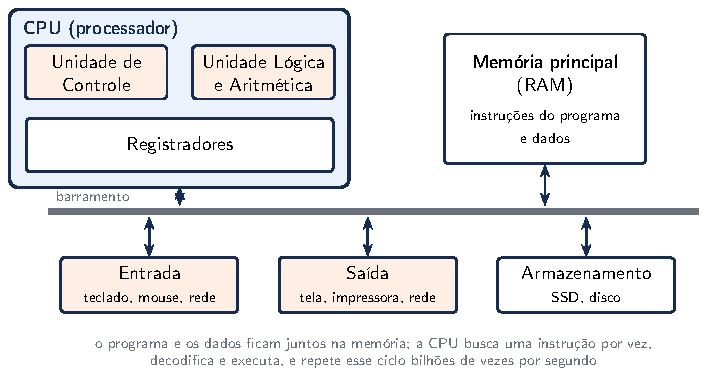
\includegraphics[width=0.95\linewidth,keepaspectratio]{imagens/capitulo-01_von-neumann.pdf}
\end{center}

\begin{itemize}
  \item A \textbf{CPU} (unidade central de processamento, ou processador) executa as instruções. A \textbf{unidade de controle} busca cada instrução e coordena a execução; a \textbf{unidade lógica e aritmética} (ULA) faz as contas e as comparações; os \textbf{registradores} são pequenas memórias dentro da CPU, extremamente rápidas, que guardam os valores em uso naquele instante.
  \item A \textbf{memória principal} (RAM) guarda o programa em execução e seus dados. É rápida, mas perde tudo quando o computador é desligado.
  \item O \textbf{armazenamento} (SSD ou disco) guarda arquivos e programas de forma permanente, mas é bem mais lento que a RAM. Para executar um programa, o sistema o copia do armazenamento para a memória.
  \item Os dispositivos de \textbf{entrada} e de \textbf{saída} trocam informações com o mundo: teclado, tela, rede.
  \item O \textbf{barramento} é o conjunto de ligações por onde os dados circulam entre essas partes.
\end{itemize}

A CPU trabalha em um ciclo que se repete sem parar: \textbf{busca} a próxima instrução na memória, \textbf{decodifica} o que ela pede e a \textbf{executa}. Um processador atual repete esse ciclo bilhões de vezes por segundo. Cada instrução, porém, é muito simples, como somar dois números, comparar dois valores ou copiar um dado de um lugar para outro. Tudo o que um programa faz, de uma planilha a um jogo, é uma sequência enorme dessas operações simples.

Dentro do computador, tudo é representado em \textbf{binário}, com apenas dois símbolos, 0 e 1. Cada um desses dígitos é um \textbf{bit}, e um grupo de 8 bits forma um \textbf{byte}, a unidade usada para medir memória e arquivos. Um byte pode representar $2^8 = 256$ valores diferentes, o suficiente para um número de 0 a 255 ou para uma letra.

Essa visão explica a sequência que todo programa segue, e que vai aparecer em todos os algoritmos desta apostila:

\begin{center}
\textbf{entrada} $\rightarrow$ \textbf{processamento} $\rightarrow$ \textbf{saída}
\end{center}

Os dados chegam pela entrada, são guardados na memória, transformados pela CPU e o resultado é enviado para a saída.

\subsection{1.4 Do problema ao algoritmo}

O erro mais comum de quem começa a programar é sair escrevendo código antes de entender o problema. Um roteiro simples evita isso:

\begin{enumerate}
  \item \textbf{Entender o problema}: o que precisa ser feito? Qual resultado se espera? Se possível, resolva um exemplo à mão.
  \item \textbf{Identificar as entradas}: quais dados o algoritmo precisa receber?
  \item \textbf{Identificar as saídas}: quais resultados ele deve produzir?
  \item \textbf{Definir o processamento}: quais cálculos e decisões transformam as entradas nas saídas?
  \item \textbf{Escrever o algoritmo}, em fluxograma ou em Portugol.
  \item \textbf{Testar à mão}, com alguns valores, antes de passar para o computador.
\end{enumerate}

Veja o roteiro aplicado a um problema do dia a dia: um grupo de amigos quer dividir a conta de um restaurante, que cobra 10\% de taxa de serviço.

\begin{center}
\begin{tabular}{@{}p{0.24\linewidth}p{0.66\linewidth}@{}}
\toprule
\rowcolor{headergray}
\tblheader{Etapa} & \tblheader{Resposta} \\
\midrule
entender & somar 10\% ao valor da conta e dividir o total entre as pessoas; com uma conta de R\$ 200 e 4 pessoas, cada uma paga R\$ 55 \\
\rowcolor{rowgray} entradas & o valor da conta e o número de pessoas \\
saída & o valor que cada pessoa paga \\
\rowcolor{rowgray} processamento & total $\leftarrow$ conta $\times$ 1,10; porPessoa $\leftarrow$ total / pessoas \\
\bottomrule
\end{tabular}
\end{center}

Repare que o exemplo resolvido à mão, na primeira linha, já serve de teste: quando o algoritmo estiver pronto, ele precisa dar R\$ 55 para essa entrada.

\subsection{1.5 Fluxogramas}

O \textbf{fluxograma} representa um algoritmo com desenhos: cada tipo de passo tem uma forma geométrica, e setas mostram a ordem. Ele é útil para enxergar o caminho do algoritmo, principalmente quando há decisões, antes de se preocupar com a escrita.

\begin{center}
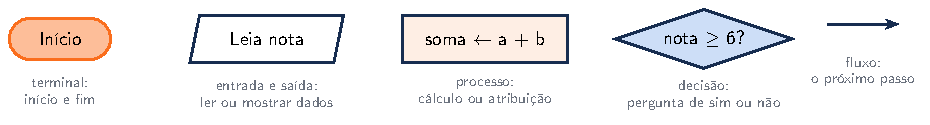
\includegraphics[width=\linewidth,keepaspectratio]{imagens/capitulo-01_simbolos.pdf}
\end{center}

O fluxograma abaixo lê duas notas, calcula a média e informa se o aluno foi aprovado. A seta $\leftarrow$ indica \textbf{atribuição}: ``media $\leftarrow$ (nota1 + nota2) / 2'' significa ``calcule (nota1 + nota2) / 2 e guarde o resultado em media''. O losango tem duas saídas, e o caminho seguido depende da resposta à pergunta.

\begin{center}
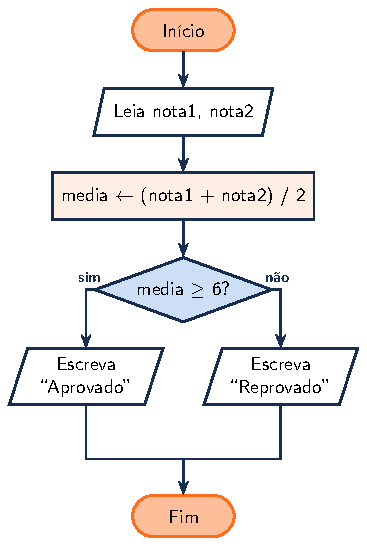
\includegraphics[width=0.5\linewidth,keepaspectratio]{imagens/capitulo-01_fluxograma-media.pdf}
\end{center}

Alguns cuidados deixam o fluxograma fácil de ler: ele tem um único início e um único fim; o fluxo corre de cima para baixo; toda decisão tem as duas saídas identificadas; e as setas não se cruzam. Para algoritmos grandes, porém, o desenho fica difícil de manter, e é aí que o pseudocódigo se torna mais prático.

\subsection{1.6 Portugol}

O \textbf{Portugol} é um \textbf{pseudocódigo} em português: uma forma estruturada de escrever algoritmos, com poucas palavras e regras fixas, mas sem os detalhes de uma linguagem de programação real. Ele permite pensar na lógica sem se preocupar com ponto e vírgula, bibliotecas ou mensagens do compilador.

Não existe um Portugol único: cada livro e cada ferramenta usa uma variação. Nesta apostila usamos a do \textbf{VisuAlg}, um programa gratuito, muito usado no ensino no Brasil, que executa algoritmos em Portugol. Assim, todo algoritmo das próximas páginas pode ser digitado e testado nele. Outra ferramenta conhecida é o Portugol Studio, que usa uma sintaxe um pouco diferente, com chaves.

Este é o algoritmo do fluxograma anterior em Portugol:

\begin{codigo}
\begin{Verbatim}[breaklines=true, breaksymbolleft={}, fontsize=\footnotesize]
algoritmo "Media"
var
   nota1, nota2, media: real
inicio
   escreva("Digite a nota 1: ")
   leia(nota1)
   escreva("Digite a nota 2: ")
   leia(nota2)
   media <- (nota1 + nota2) / 2
   se media >= 6 entao
      escreval("Aprovado! Média: ", media)
   senao
      escreval("Reprovado. Média: ", media)
   fimse
fimalgoritmo
\end{Verbatim}
\end{codigo}

\begin{itemize}
  \item \texttt{algoritmo "Media"} dá um nome ao algoritmo.
  \item Em \texttt{var} são declaradas as \textbf{variáveis}, os espaços da memória onde os dados ficam guardados, cada uma com seu \textbf{tipo}: \texttt{inteiro}, \texttt{real} (com casas decimais), \texttt{caractere} (texto) ou \texttt{logico} (verdadeiro ou falso). O Capítulo 3 trata disso em detalhe.
  \item Entre \texttt{inicio} e \texttt{fimalgoritmo} ficam os comandos, executados de cima para baixo.
  \item \texttt{leia} recebe um valor digitado; \texttt{escreva} mostra um texto ou valor na tela, e \texttt{escreval} faz o mesmo e pula para a linha seguinte.
  \item \texttt{<-} é a atribuição, a mesma seta do fluxograma.
  \item \texttt{se ... entao ... senao ... fimse} escolhe entre dois caminhos, como o losango.
\end{itemize}

O recuo das linhas internas não é obrigatório, mas mostra visualmente o que está dentro de quê. Acostume-se a usá-lo desde já: em C++ ele vai ser igualmente importante para a leitura.

O algoritmo da conta do restaurante, da Seção 1.4, fica assim:

\begin{codigo}
\begin{Verbatim}[breaklines=true, breaksymbolleft={}, fontsize=\footnotesize]
algoritmo "DividirConta"
var
   conta, total, porPessoa: real
   pessoas: inteiro
inicio
   escreva("Valor da conta: ")
   leia(conta)
   escreva("Número de pessoas: ")
   leia(pessoas)
   total <- conta * 1.10            // 10% de serviço
   porPessoa <- total / pessoas
   escreval("Cada pessoa paga R$ ", porPessoa)
fimalgoritmo
\end{Verbatim}
\end{codigo}

O que vem depois de \texttt{//} é um \textbf{comentário}: uma anotação para quem lê, que não é executada. Note também que, no Portugol e nas linguagens de programação, o separador decimal é o \textbf{ponto}, e não a vírgula: \texttt{1.10}, e não \texttt{1,10}.

\subsubsection{Teste de mesa}

O \textbf{teste de mesa} é a forma de testar um algoritmo sem computador: você executa os passos no papel, anotando em uma tabela o valor de cada variável a cada linha. Ele revela erros de lógica antes mesmo de o programa existir. Para o algoritmo da média, vale testar um caso de cada resultado e o valor exatamente na fronteira, 6:

\begin{center}
\begin{tabular}{@{}p{0.14\linewidth}p{0.14\linewidth}p{0.14\linewidth}p{0.42\linewidth}@{}}
\toprule
\rowcolor{headergray}
\tblheader{nota1} & \tblheader{nota2} & \tblheader{media} & \tblheader{Saída} \\
\midrule
7.0 & 4.0 & 5.5 & Reprovado \\
\rowcolor{rowgray} 8.0 & 9.0 & 8.5 & Aprovado \\
6.0 & 6.0 & 6.0 & Aprovado (a condição é \texttt{>=}) \\
\bottomrule
\end{tabular}
\end{center}

Se o algoritmo tivesse sido escrito com \texttt{>} no lugar de \texttt{>=}, a terceira linha mostraria o erro: um aluno com média exatamente 6 seria reprovado.

\subsection{1.7 Do Portugol ao C++}

O Portugol ajuda a pensar, mas o computador não o entende diretamente. Para que o algoritmo vire um programa, ele precisa ser escrito em uma \textbf{linguagem de programação}. Nesta disciplina usamos o \textbf{C++}, uma das linguagens mais usadas no mundo, presente em sistemas operacionais, jogos, navegadores e bancos de dados. Veja o algoritmo da média em C++, lado a lado com o que você já conhece:

\begin{codigo}
\begin{Verbatim}[breaklines=true, breaksymbolleft={}, fontsize=\footnotesize]
#include <iostream>
using namespace std;

int main() {
    double nota1, nota2, media;       // var ... : real
    cout << "Digite a nota 1: ";      // escreva
    cin >> nota1;                     // leia
    cout << "Digite a nota 2: ";
    cin >> nota2;
    media = (nota1 + nota2) / 2;      // media <- ...
    if (media >= 6) {                 // se ... entao
        cout << "Aprovado! Média: " << media << endl;
    } else {                          // senao
        cout << "Reprovado. Média: " << media << endl;
    }                                 // fimse
    return 0;
}
\end{Verbatim}
\end{codigo}

A estrutura é a mesma; mudam as palavras e alguns sinais. As principais correspondências:

\begin{center}
\begin{tabular}{@{}p{0.4\linewidth}p{0.5\linewidth}@{}}
\toprule
\rowcolor{headergray}
\tblheader{Portugol} & \tblheader{C++} \\
\midrule
\texttt{inicio} ... \texttt{fimalgoritmo} & \texttt{int main() \{} ... \texttt{\}} \\
\rowcolor{rowgray} \texttt{real}, \texttt{inteiro} & \texttt{double}, \texttt{int} \\
\texttt{leia(x)} & \texttt{cin >> x;} \\
\rowcolor{rowgray} \texttt{escreva(x)} & \texttt{cout << x;} \\
\texttt{x <- 5} & \texttt{x = 5;} \\
\rowcolor{rowgray} \texttt{se} ... \texttt{entao} ... \texttt{fimse} & \texttt{if (...) \{} ... \texttt{\}} \\
\bottomrule
\end{tabular}
\end{center}

Não se preocupe ainda com o \texttt{\#include}, o \texttt{using namespace std} e o ponto e vírgula no fim das linhas: o Capítulo 2 explica cada parte de um programa em C++, como ele é transformado em algo que o computador executa e como montar o seu ambiente para programar.

\subsection{Erros Comuns}

\begin{itemize}
  \item \textbf{Começar pelo código.} Sem entender o problema e identificar entradas e saídas, o programa resolve o problema errado. Siga o roteiro da Seção 1.4.
  \item \textbf{Escrever passos ambíguos.} ``Calcule o desconto'' não diz qual desconto nem sobre qual valor. Cada passo precisa ser executável sem que ninguém precise adivinhar nada.
  \item \textbf{Criar um algoritmo que nunca termina.} ``Repita até a água ferver'' sem um fogão ligado não acaba. Toda repetição precisa de uma condição que um dia se torne falsa.
  \item \textbf{Confundir E com OU.} ``Nota maior ou igual a 6 \textbf{ou} frequência maior ou igual a 75\%'' aprova quem só cumpriu uma das exigências.
  \item \textbf{Esquecer um dos caminhos da decisão.} Todo losango tem duas saídas. Pergunte sempre: e se a resposta for não?
  \item \textbf{Confundir atribuição com igualdade.} \texttt{media <- 6} guarda 6 em \texttt{media}; não é uma pergunta. A comparação ``media é igual a 6?'' é escrita de outra forma, como você verá no Capítulo 3.
  \item \textbf{Usar vírgula como separador decimal.} No Portugol e no C++, escreve-se \texttt{1.10}.
  \item \textbf{Testar só o caso fácil.} Inclua no teste de mesa os valores de fronteira, como a média exatamente 6.
\end{itemize}
